\documentclass{article}
\usepackage{fancyhdr}
\usepackage{ctex}
\usepackage{listings}
\usepackage{graphicx}
\usepackage[a4paper, body={18cm,22cm}]{geometry}
\usepackage{amsmath,amssymb,amstext,wasysym,enumerate,graphicx}
\usepackage{float,abstract,booktabs,indentfirst,amsmath}
\usepackage{array}
\usepackage{booktabs}
\usepackage{multirow}
\usepackage{url}
\usepackage{diagbox}
\usepackage{hyperref}
\usepackage{listings}
\renewcommand\arraystretch{1.4}
\usepackage{indentfirst}
\setlength{\parindent}{2em}
\usepackage{enumitem}
\usepackage{accsupp}
\setmonofont{Consolas}
\usepackage{listings}
\usepackage{xcolor}
\usepackage{makecell}
\usepackage{subfigure}
\usepackage{longtable}
\setCJKmonofont{黑体}
\newcommand\emptyaccsupp[1]{\BeginAccSupp{ActualText={}}#1\EndAccSupp{}}
\newcommand\SQL{\texttt{SQL}}
\renewcommand\tt{\texttt}
\lstset{
    % language = C,
    showstringspaces=false,
    xleftmargin = 3em,xrightmargin = 3em, aboveskip = 1em,
	backgroundcolor = \color{white}, % 背景色
	basicstyle = \small\ttfamily, % 基本样式 + 小号字体
	rulesepcolor= \color{gray}, % 代码块边框颜色
	breaklines = true, % 代码过长则换行
	numbers = left, % 行号在左侧显示
	numberstyle=\emptyaccsupp,
    numbersep = 14pt, 
    keywordstyle=\color{purple}\bfseries, % 关键字颜色
    commentstyle =\color{red!50!green!50!blue!60}, % 注释颜色
    stringstyle = \color{red}, % 字符串颜色
    morekeywords={ASSERT, int64_t, uint32_t},
	% frame = shadowbox, % 用(带影子效果)方框框住代码块
	frame = single, % 用(带影子效果)方框框住代码块
	showspaces = false, % 不显示空格
	columns = fixed, % 字间距固定
  framesep=1em
} 
\lstset{
    sensitive=true,
    moreemph={ASSERT, NULL}, emphstyle=\color{red}\bfseries,
    moreemph=[2]{int64_t, uint32_t, tid_t, uint8_t, int16_t, uint16_t, int32_t, size_t}, emphstyle=[2]\color{purple}\bfseries,
    showspaces = false, % 不显示空格
    }
%--------------------页眉--------------------%
\pagestyle{fancy}
\fancyhead[L]{}
\fancyhead[R]{}
\fancyhead[C]{《数据库系统及应用实践》课程实验报告}
\fancyfoot[C]{-\thepage-}
\renewcommand{\headrulewidth}{1.5pt}
%--------------------标题--------------------%
\begin{document}
\begin{center}
  \LARGE{{\textbf{\heiti 《数据库系统及应用实践》课程实验报告}}}

  \vspace{0.5em}

  \large 实验5:存储、索引和基准测试
  \begin{table}[H]
    \centering
    \begin{tabular}{p{2cm}p{2cm}<{\centering}p{0.4cm}p{2cm}p{3cm}<{\centering}p{0.4cm}p{2cm}p{3cm}<{\centering}}
      姓\qquad 名: & 李鹏达 & \quad & 学\qquad 号: & 10225101460 & \quad & 完成日期: & 2024年5月16日 \\ \cline{2-2} \cline{5-5} \cline{8-8}
    \end{tabular}
  \end{table}
\end{center}
% \rule{\textwidth}{1pt}
%--------------------正文--------------------%
\section{实验目标}
\begin{enumerate}[noitemsep]
  \item 学习和理解MySQL数据库管理系统中表空间、模式和索引的基本概念和操作;
  \item 理解MySQL数据库管理系统中数据存储的基本结构;
  \item 了解索引对查询性能的影响,能够根据应用场景设计合适的索引;
  \item 使用TPC-H基准测试对MySQL数据库管理系统进行评测;
\end{enumerate}

\section{实验过程记录}

在 Docker 容器中启动 MySQL 数据库,并连接到数据库 \tt{dbcourse}。

\subsection{表空间管理}

执行以下SQL语句,创建一个名为\tt{myspace}的表空间;

\begin{lstlisting}[language=sql]
create tablespace myspace add datafile 'myspace.ibd';
\end{lstlisting}

运行结果如下:

\begin{figure}[H]
\centering
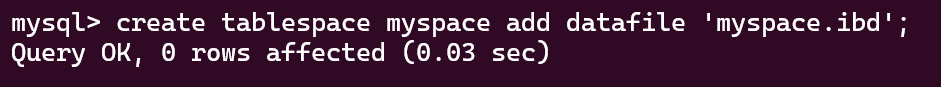
\includegraphics[width=0.9\textwidth]{img/1.png}
\caption{创建表空间}
\end{figure}

执行以下SQL语句,在\tt{myspace}表空间中创建数据表\tt{t1};

\begin{lstlisting}[language=sql]
create table t1(c1 int primary key, c2 varchar(10)) tablespace myspace;
\end{lstlisting}

运行结果如下:

\begin{figure}[H]
\centering
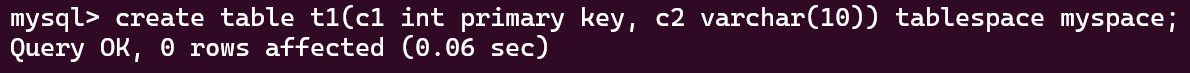
\includegraphics[width=0.9\textwidth]{img/2.png}
\caption{在表空间中创建数据表}
\end{figure}

执行以下SQL语句,在\tt{System Tablespace}, \tt{File-Per-Table Tablespace}和\tt{General Tablespace}之间迁移数据表;

\begin{lstlisting}[language=sql]
alter table advisor tablespace myspace;
alter table classroom tablespace innodb_system;
alter table t1 tablespace innodb_file_per_table;
\end{lstlisting}

运行结果如下:

\begin{figure}[H]
\centering
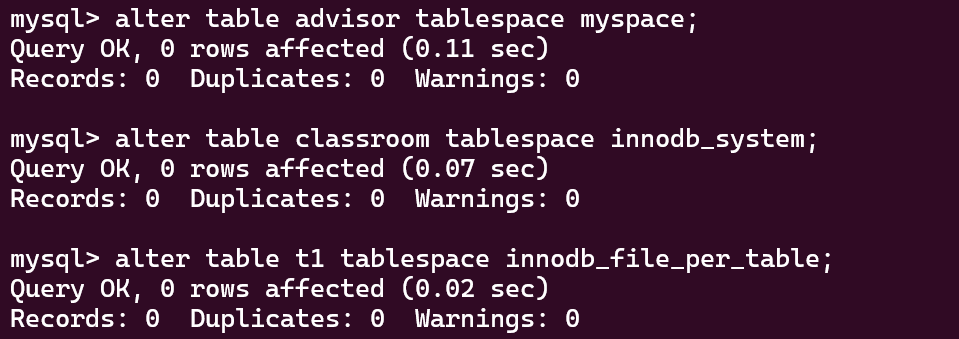
\includegraphics[width=0.7\textwidth]{img/3.png}
\caption{迁移数据表}
\end{figure}

执行以下SQL语句,查询系统中的表空间信息;

\begin{lstlisting}[language=sql]
select space, name, space_type, file_size from information_schema.innodb_tablespaces;
\end{lstlisting}

运行结果如下:

\begin{figure}[H]
\centering
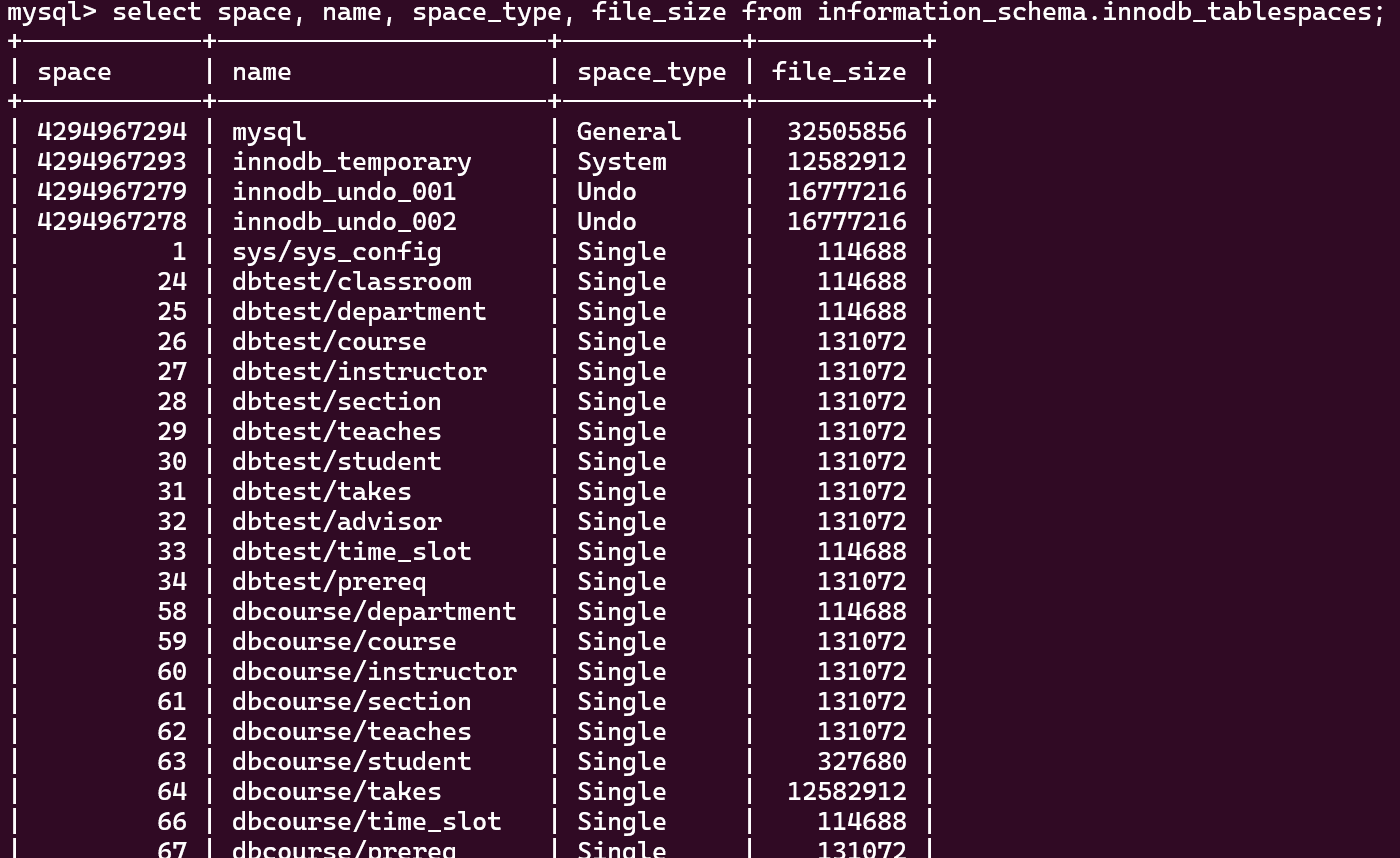
\includegraphics[width=0.65\textwidth]{img/4.png}
\caption{查询表空间信息}
\end{figure}

执行以下SQL语句,查询系统中数据表在表空间的分布情况;

\begin{lstlisting}[language=sql]
select ts.name as tablespaces, t.name as tables from information_schema.innodb_tablespaces ts, information_schema.innodb_tables t where ts.space = t.space;
\end{lstlisting}

运行结果如下:

\begin{figure}[H]
\centering
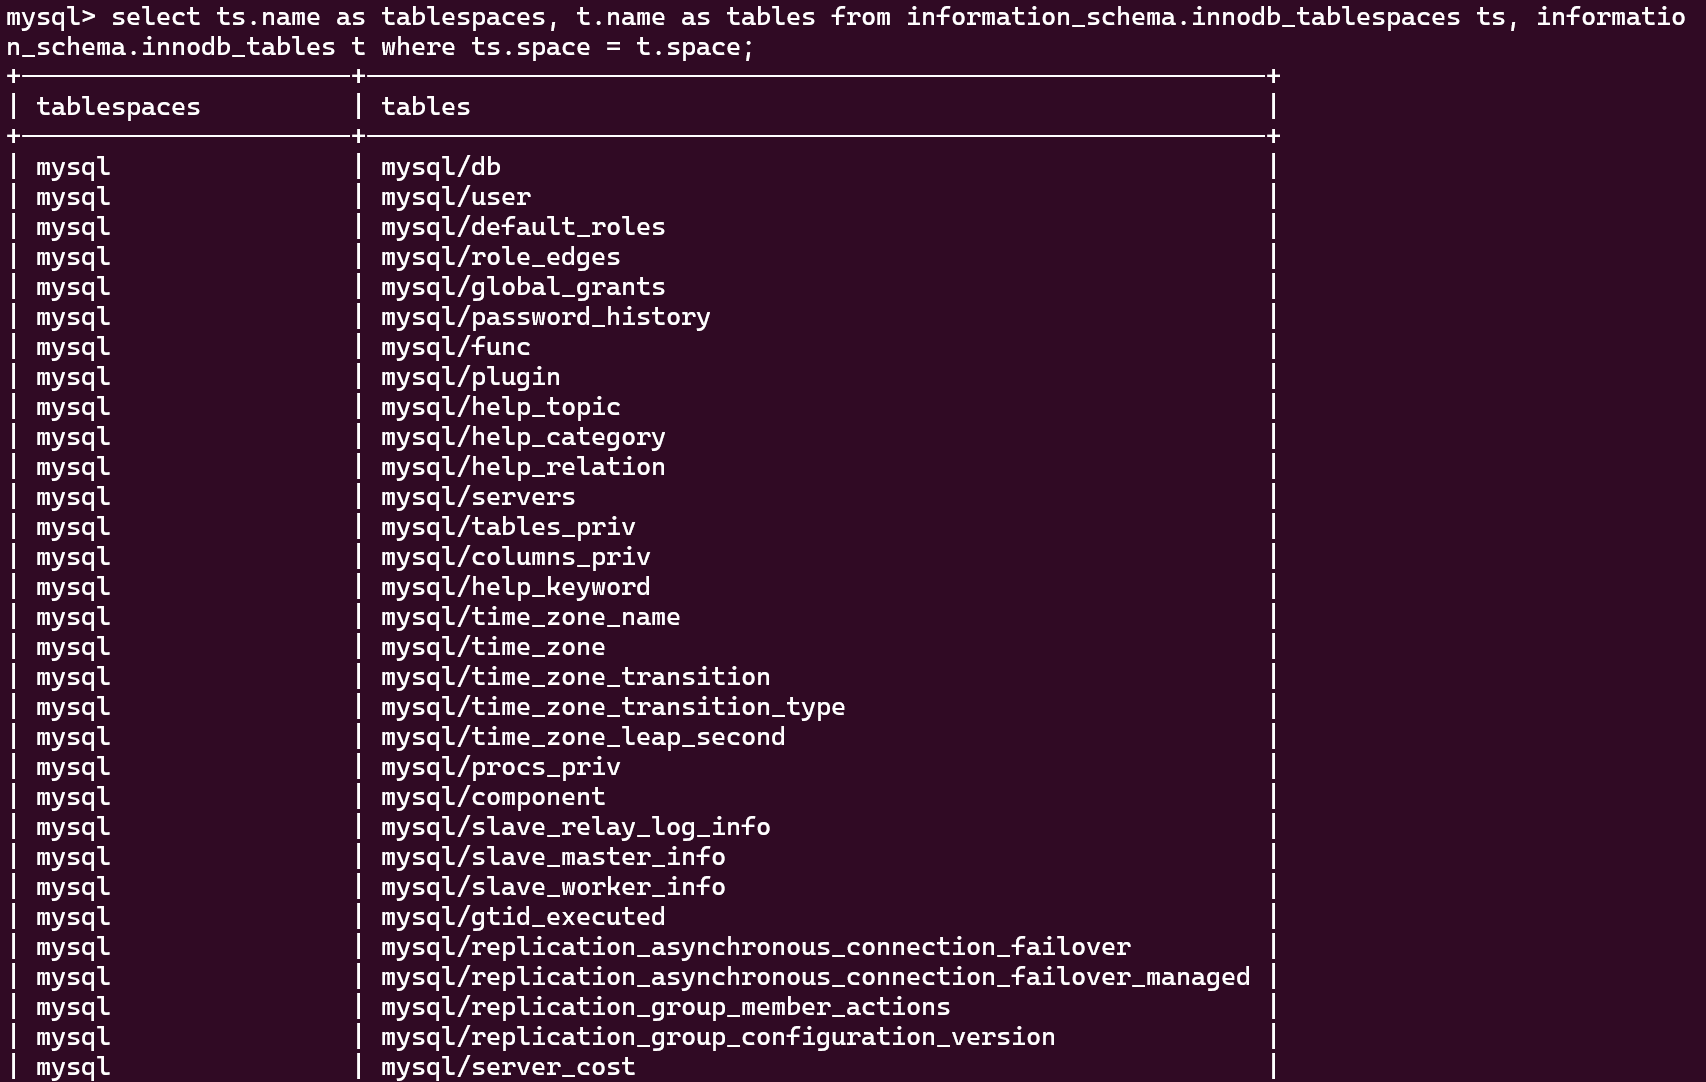
\includegraphics[width=0.9\textwidth]{img/5.png}
\caption{查询数据表在表空间的分布情况}
\end{figure}

执行以下SQL语句,将表空间\tt{myspace}改名为\tt{tablespace\_460};

\begin{lstlisting}[language=sql]
alter tablespace myspace rename to tablespace_460;
\end{lstlisting}

运行结果如下:

\begin{figure}[H]
\centering
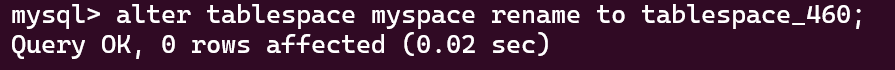
\includegraphics[width=0.9\textwidth]{img/6.png}
\caption{将表空间改名}
\end{figure}

执行以下SQL语句,删除表空间\tt{tablespace\_460};

\begin{lstlisting}[language=sql]
alter table advisor tablespace innodb_system;
drop tablespace tablespace_460;
\end{lstlisting}

运行结果如下:

\begin{figure}[H]
\centering
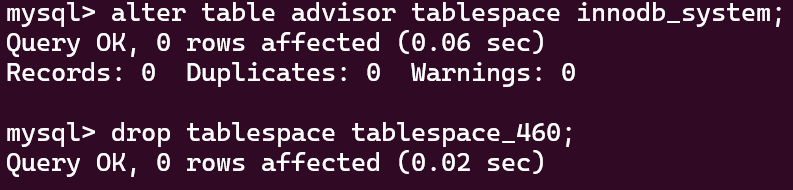
\includegraphics[width=0.5\textwidth]{img/7.png}
\caption{删除表空间}
\end{figure}

\subsection{模式}

执行下列SQL语句,练习在查询中使用模式;

\begin{lstlisting}[language=sql]
select * from movies;
select * from movie.movies;
use movie;
select * from movies;
use dbcourse;
\end{lstlisting}

运行结果如下:

\begin{figure}[H]
\centering
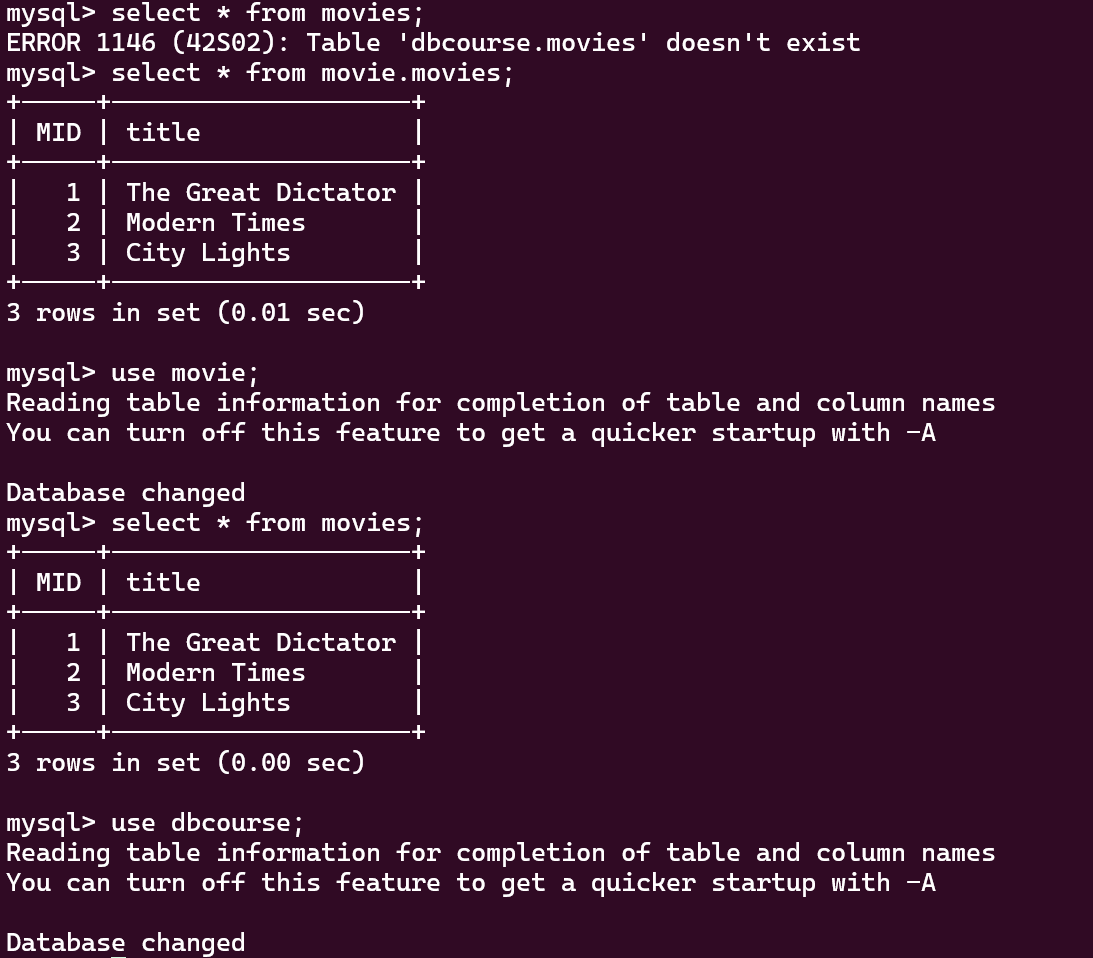
\includegraphics[width=0.56\textwidth]{img/8.png}
\caption{使用模式}
\end{figure}

\subsection{索引管理}

下载实验所需的数据文件(*.tbl),并将其复制到容器中的 \tt{/dbcourse} 文件夹中;

\begin{lstlisting}[language=bash]
unzip tbl.zip
for file in *.tbl; do
  sudo docker cp "$file" "dbcourse:/dbcourse/$file"
done
\end{lstlisting}

执行以下SQL语句,创建数据表\tt{tpch};

\begin{lstlisting}[language=sql]
CREATE DATABASE tpch CHARACTER SET utf8mb4;
USE tpch;
CREATE TABLE nation(n_nationKEY INTEGER PRIMARY KEY, n_name CHAR(25) NOT NULL, n_regionkey INTEGER NOT NULL, n_comment VARCHAR(152));
CREATE TABLE region(r_regionkey INTEGER PRIMARY KEY, r_name CHAR(25) NOT NULL, r_comment VARCHAR(152));
CREATE TABLE part(p_partkey INTEGER PRIMARY KEY, p_name VARCHAR(55) NOT NULL, p_mfgr CHAR(25) NOT NULL, p_brand CHAR(10) NOT NULL, p_type VARCHAR(25) NOT NULL, p_size INTEGER NOT NULL, p_container CHAR(10) NOT NULL, p_retailprice DECIMAL(15,2) NOT NULL, p_comment VARCHAR(23) NOT NULL);
CREATE TABLE supplier(s_suppkey INTEGER PRIMARY KEY, s_name CHAR(25) NOT NULL, s_address VARCHAR(40) NOT NULL, s_nationkey INTEGER NOT NULL, s_phone CHAR(15) NOT NULL, s_acctbal DECIMAL(15,2) NOT NULL, s_comment VARCHAR(101) NOT NULL);
CREATE TABLE partsupp(ps_partkey INTEGER NOT NULL, ps_suppkey INTEGER NOT NULL, ps_availqty INTEGER NOT NULL, ps_supplycost DECIMAL(15,2) NOT NULL, ps_comment VARCHAR(199) NOT NULL, PRIMARY KEY (ps_partkey, ps_suppkey) );
CREATE TABLE customer(c_custkey INTEGER PRIMARY KEY, c_name VARCHAR(25) NOT NULL, c_address VARCHAR(40) NOT NULL, c_nationkey INTEGER NOT NULL, c_phone CHAR(15) NOT NULL, c_acctbal DECIMAL(15,2) NOT NULL, c_mktsegment CHAR(10) NOT NULL, c_comment VARCHAR(117) NOT NULL);
CREATE TABLE orders(o_orderkey INTEGER PRIMARY KEY, o_custkey INTEGER NOT NULL, o_orderstatus CHAR(1) NOT NULL, o_totalprice DECIMAL(15,2) NOT NULL, o_orderdate date NOT NULL, o_orderpriority CHAR(15) NOT NULL, o_clerk CHAR(15) NOT NULL, o_shippriority INTEGER NOT NULL, o_comment VARCHAR(79) NOT NULL);
CREATE TABLE lineitem(l_orderkey INTEGER NOT NULL, l_partkey INTEGER NOT NULL, l_suppkey INTEGER NOT NULL, l_linenumber INTEGER NOT NULL, l_quantity DECIMAL(15,2) NOT NULL, l_extendedprice DECIMAL(15,2) NOT NULL, l_discount DECIMAL(15,2) NOT NULL, l_tax DECIMAL(15,2) NOT NULL, l_returnflag CHAR(1) NOT NULL, l_linestatus CHAR(1) NOT NULL, l_shipdate date NOT NULL, l_commitdate date NOT NULL, l_receiptdate date NOT NULL, l_shipinstruct CHAR(25) NOT NULL, l_shipmode CHAR(10) NOT NULL, l_comment VARCHAR(44) NOT NULL, PRIMARY KEY(l_orderkey,l_linenumber));
\end{lstlisting}

部分运行结果如下:

\begin{figure}[H]
\centering
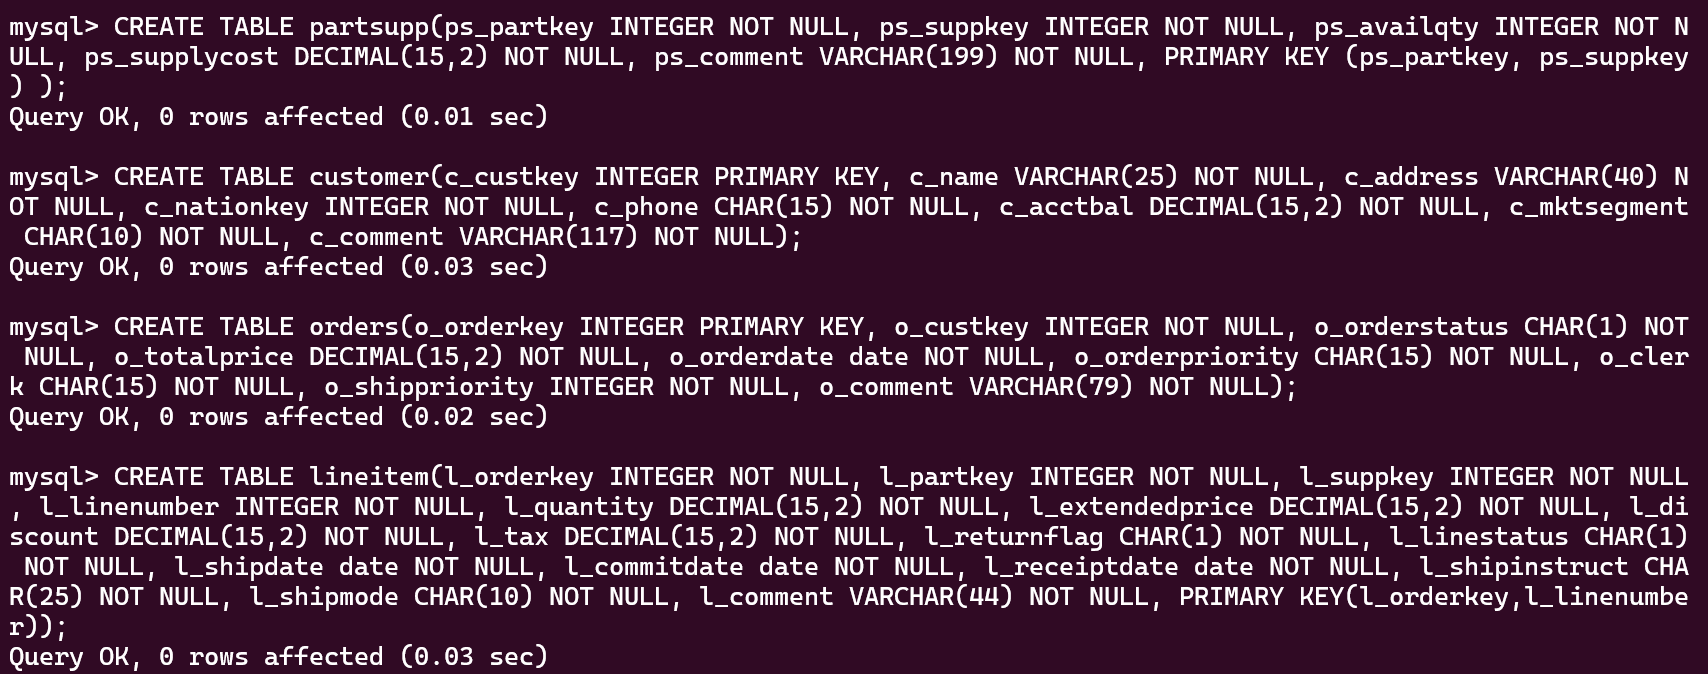
\includegraphics[width=0.9\textwidth]{img/9.png}
\caption{创建数据表}
\end{figure}

执行下列命令/语句,修改系统配置,允许从MySQL客户端加载数据;

\begin{lstlisting}[language=bash]
show global variables like 'local_infile';
set global local_infile = on;
show global variables like 'local_infile';
quit
mysql --local-infile=1 -uroot -p -Dtpch
\end{lstlisting}

\begin{figure}[H]
\centering
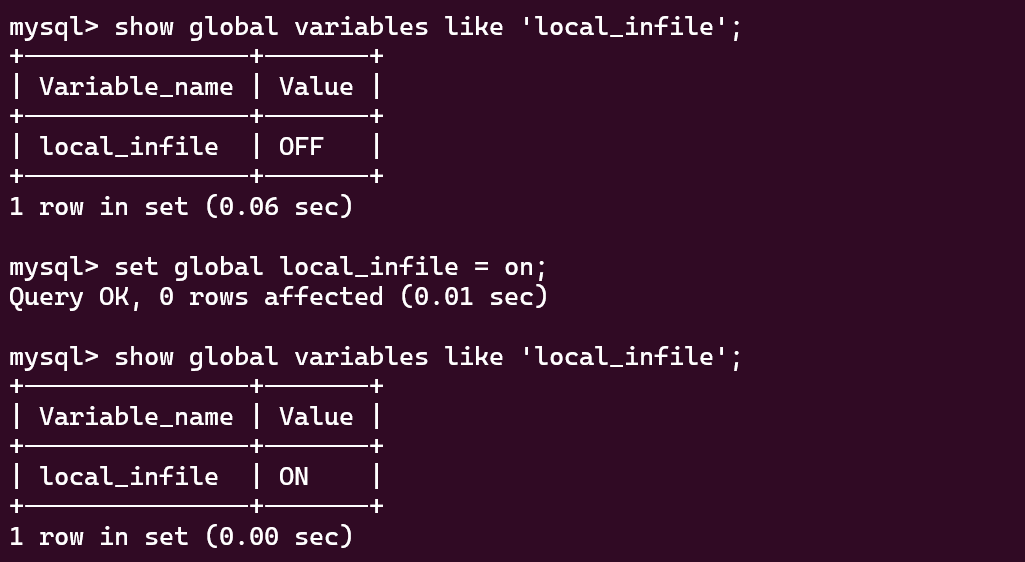
\includegraphics[width=0.75\textwidth]{img/10.png}
\caption{修改系统配置}
\end{figure}

执行下列命令,从客户端本地数据文件中导入数据;

\begin{lstlisting}[language=sql]
load data local infile '/dbcourse/nation.tbl' into table nation fields terminated by '|' lines terminated by '\n';
load data local infile '/dbcourse/region.tbl' into table region fields terminated by '|' lines terminated by '\n';
load data local infile '/dbcourse/part.tbl' into table part fields terminated by '|' lines terminated by '\n';
load data local infile '/dbcourse/supplier.tbl' into table supplier fields terminated by '|' lines terminated by '\n';
load data local infile '/dbcourse/partsupp.tbl' into table partsupp fields terminated by '|' lines terminated by '\n';
load data local infile '/dbcourse/customer.tbl' into table customer fields terminated by '|' lines terminated by '\n';
load data local infile '/dbcourse/orders.tbl' into table orders fields terminated by '|' lines terminated by '\n';
load data local infile '/dbcourse/lineitem.tbl' into table lineitem fields terminated by '|' lines terminated by '\n';
\end{lstlisting}

部分运行结果如下:

\begin{figure}[H]
\centering
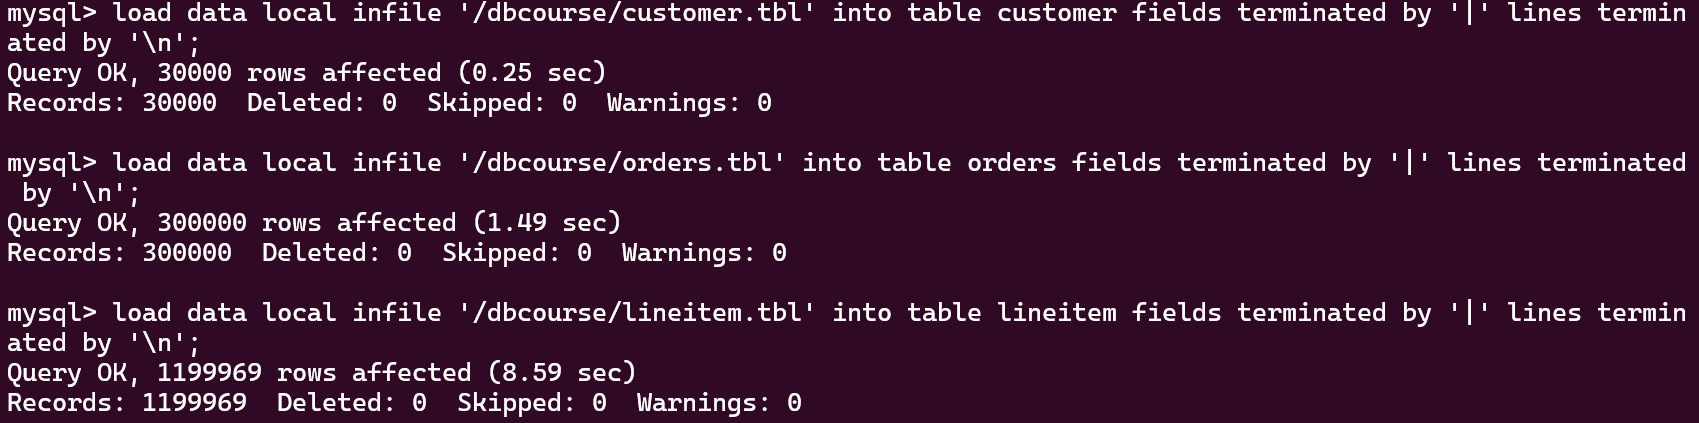
\includegraphics[width=0.9\textwidth]{img/11.png}
\caption{导入数据}
\end{figure}

修改会话变量 \tt{profiling},允许统计当前会话中每条语句的资源消耗情况;

\begin{lstlisting}[language=sql]
show variables like 'profiling';
set profiling = on;
show variables like 'profiling';
\end{lstlisting}

如图所示:

\begin{figure}[H]
\centering
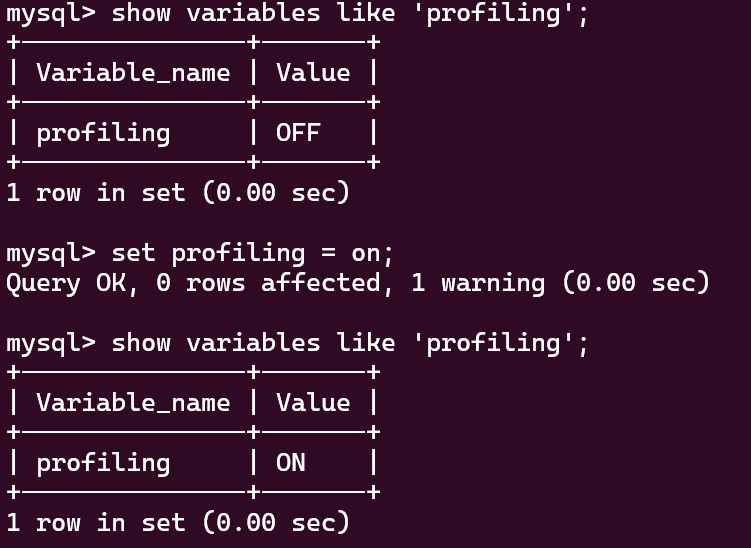
\includegraphics[width=0.5\textwidth]{img/12.png}
\caption{修改会话变量}
\end{figure}

执行下列语句,对比两个查询的资源消耗情况,记录并分析相关数据;

\begin{lstlisting}[language=sql]
select * from lineitem;
show profile;
select l_orderkey, l_partkey, l_suppkey, l_linenumber, l_quantity,l_extendedprice, l_discount, l_tax, l_returnflag, l_linestatus, l_shipdate, l_commitdate, l_receiptdate, l_shipinstruct, l_shipmode, l_comment from lineitem;
show profile;
show profiles;
\end{lstlisting}

\begin{figure}[H]
  \centering
  \subfigure[查询1]{
    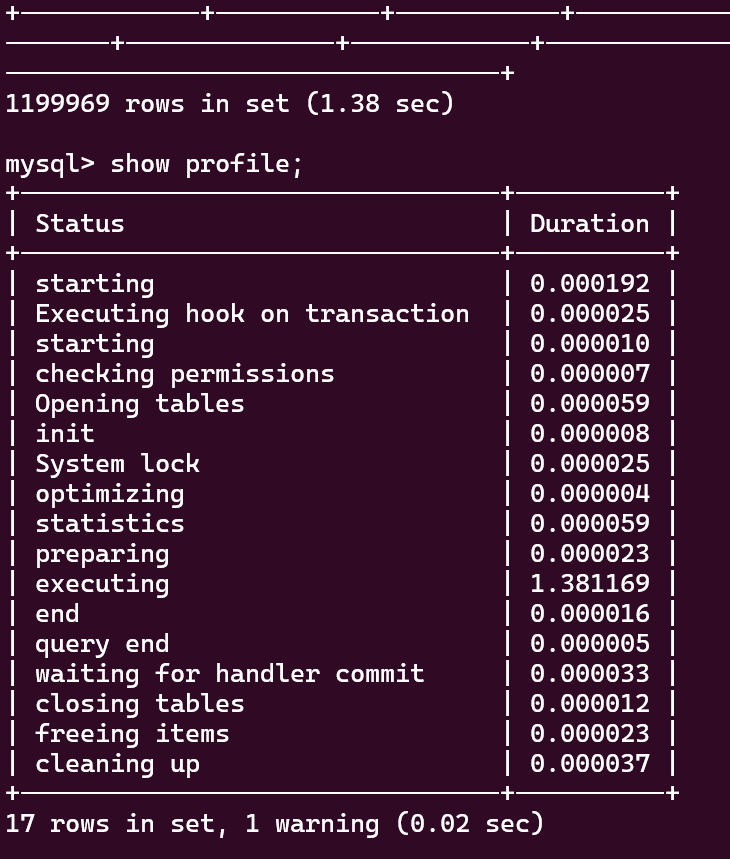
\includegraphics[width=0.3\textwidth]{img/13.png}
  }
  \subfigure[查询2]{
    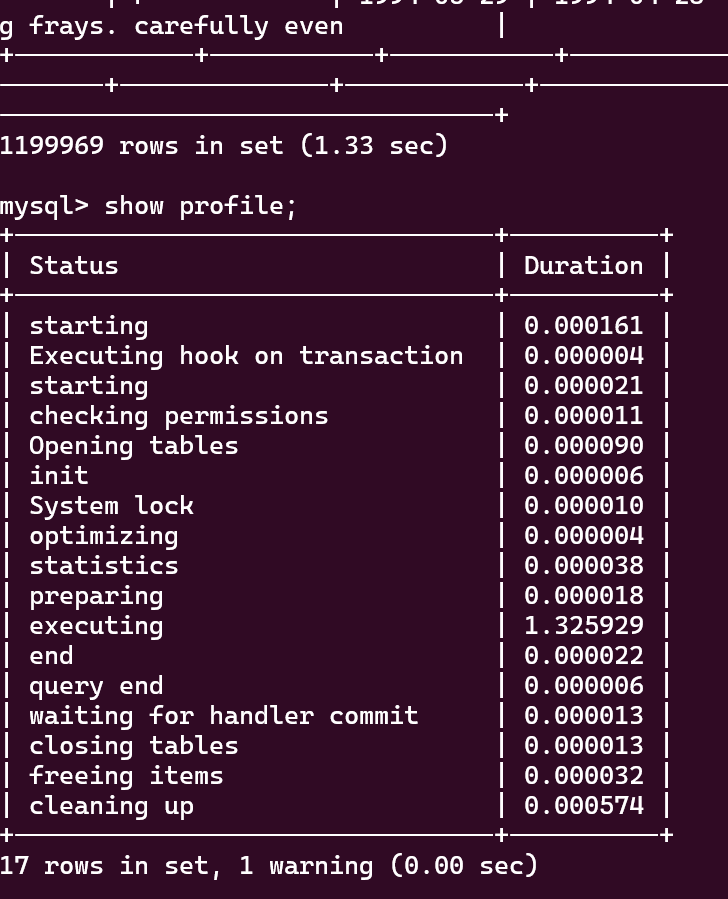
\includegraphics[width=0.3\textwidth]{img/14.png}
  }
  \caption{查询资源消耗情况}
\end{figure}

\begin{figure}
\centering
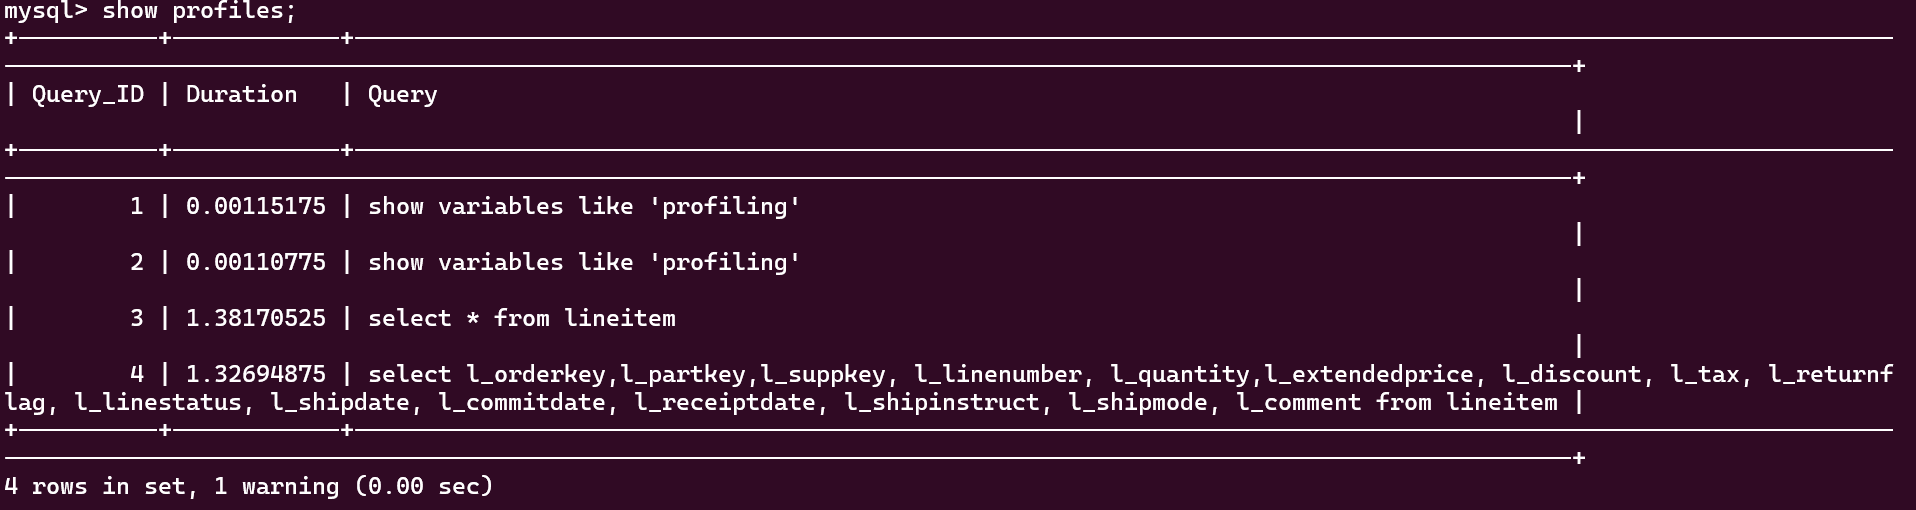
\includegraphics[width=0.9\textwidth]{img/15.png}
\caption{查询资源消耗情况比较}
\end{figure}

可以看到,查询2的资源消耗情况与查询1几乎相同,这是因为查询2和查询1均查询了整个数据表中的所有列,因此资源消耗情况相差不大。

执行下列语句,观察主键查询的性能,记录并分析相关数据;

\begin{lstlisting}[language=sql]
select * from lineitem where l_orderkey = 354 and l_linenumber = 7;
select * from lineitem where l_orderkey = 354;
select * from lineitem where l_linenumber = 7;
show profiles;
\end{lstlisting}

结果如下:

\begin{figure}[H]
\centering
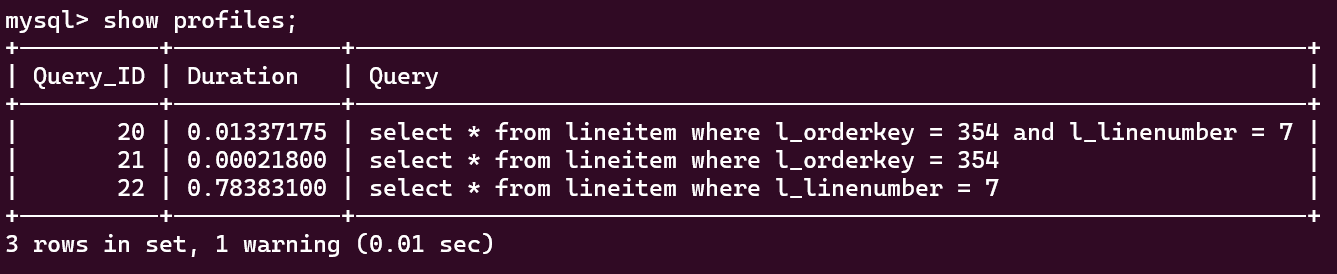
\includegraphics[width=0.9\textwidth]{img/16.png}
\caption{主键查询性能}
\end{figure}

根据分析,查询 1 和查询 2 的执行时间非常短,表明它们能够有效利用复合主键索引。而查询 3 的执行时间较长,因为它使用的是复合索引的第二项,不能利用主键索引,可能需要全表扫描。

执行下列语句,观察索引对查询性能的影响,记录并分析相关数据;

\begin{lstlisting}[language=sql]
select * from lineitem where l_partkey = 860;
create index lineitem_partkey on lineitem(l_partkey);
select * from lineitem where l_partkey = 860;
show profiles;
drop index lineitem_partkey on lineitem;
\end{lstlisting}

结果如下:

\begin{figure}[H]
\centering
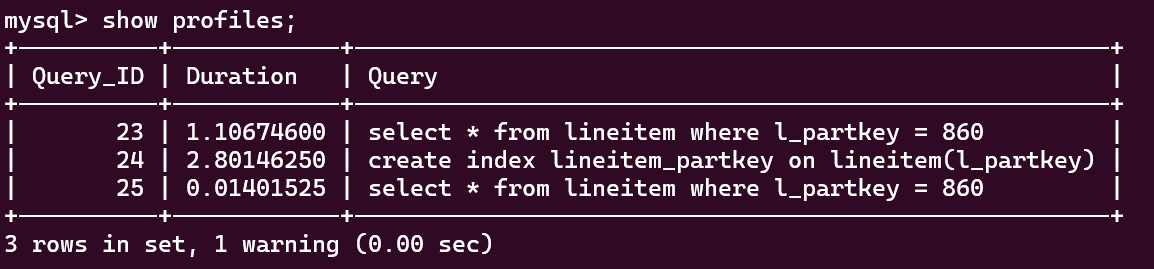
\includegraphics[width=0.9\textwidth]{img/17.png}
\caption{索引对查询性能的影响}
\end{figure}

根据分析,创建索引后,查询的执行时间明显减少,表明索引对查询性能有显著的提升。

执行下列语句,观察唯一索引、前缀索引对查询性能的影响,记录并分析相关数据;

\begin{lstlisting}[language=sql]
select * from customer where c_address = 'KvpyuHCplrB84WgAiGV6sYpZq7Tj';
select * from customer where c_address like 'KvpyuH%';
create index customer_address on customer(c_address);
select * from customer where c_address = 'KvpyuHCplrB84WgAiGV6sYpZq7Tj';
select * from customer where c_address like 'KvpyuH%';
drop index customer_address on customer;
create unique index customer_address on customer(c_address);
select * from customer where c_address = 'KvpyuHCplrB84WgAiGV6sYpZq7Tj';
select * from customer where c_address like 'KvpyuH%';
drop index customer_address on customer;
create index customer_address on customer(c_address(4));
select * from customer where c_address = 'KvpyuHCplrB84WgAiGV6sYpZq7Tj';
select * from customer where c_address like 'KvpyuH%';
show profiles;
drop index customer_address on customer;
\end{lstlisting}

结果如下:

\begin{figure}[H]
\centering
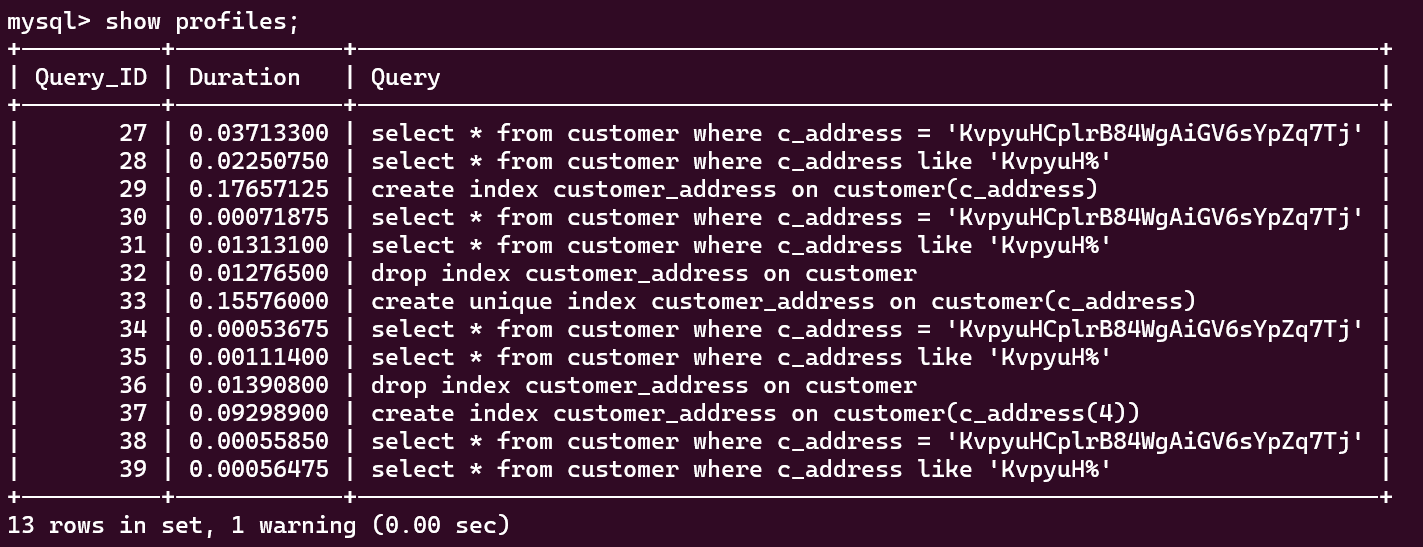
\includegraphics[width=0.9\textwidth]{img/18.png}
\caption{唯一索引、前缀索引对查询性能的影响}
\end{figure}

从查询结果和执行时间分析来看,创建索引后,查询性能显著提升,尤其是在精确匹配查询中表现突出。而对于 \tt{LIKE} 查询,前缀索引的性能更优,因为在这个场景下,\tt{LIKE} 查询匹配的区域恰好是前缀索引的索引区域。

执行下列语句,观察索引对于更新性能的影响,记录并分析相关数据;

\begin{lstlisting}[language=sql]
insert into customer values(30001,'Customer#000030001','314hjafd2354',8,'27-147-574-1234',888.88,'AUTOMOBILE','This is a test!');
update customer set c_address = 'kqe34gqerl' where c_custkey = 30001;
delete from customer where c_custkey = 30001;
show profiles;
create index customer_2 on customer(c_name);
create index customer_3 on customer(c_address);
create index customer_4 on customer(c_nationkey);
create index customer_5 on customer(c_phone);
create index customer_6 on customer(c_acctbal);
create index customer_7 on customer(c_mktsegment);
create index customer_8 on customer(c_comment);
create index customer_23 on customer(c_name,c_address);
create index customer_24 on customer(c_name,c_nationkey);
create index customer_25 on customer(c_name,c_phone);
create index customer_26 on customer(c_name,c_acctbal);
create index customer_27 on customer(c_name,c_mktsegment);
create index customer_28 on customer(c_name,c_comment);
insert into customer values(30001,'Customer#000030001','314hjafd2354',8,'27-147-574-1234',888.88,'AUTOMOBILE','This is a test!');
update customer set c_address = 'kqe34gqerl' where c_custkey = 30001;
delete from customer where c_custkey = 30001;
show profiles;
drop index customer_2 on customer;
drop index customer_3 on customer;
drop index customer_4 on customer;
drop index customer_5 on customer;
drop index customer_6 on customer;
drop index customer_7 on customer;
drop index customer_8 on customer;
drop index customer_23 on customer;
drop index customer_24 on customer;
drop index customer_25 on customer;
drop index customer_26 on customer;
drop index customer_27 on customer;
drop index customer_28 on customer;
\end{lstlisting}

结果如下:

\begin{figure}[H]
\centering
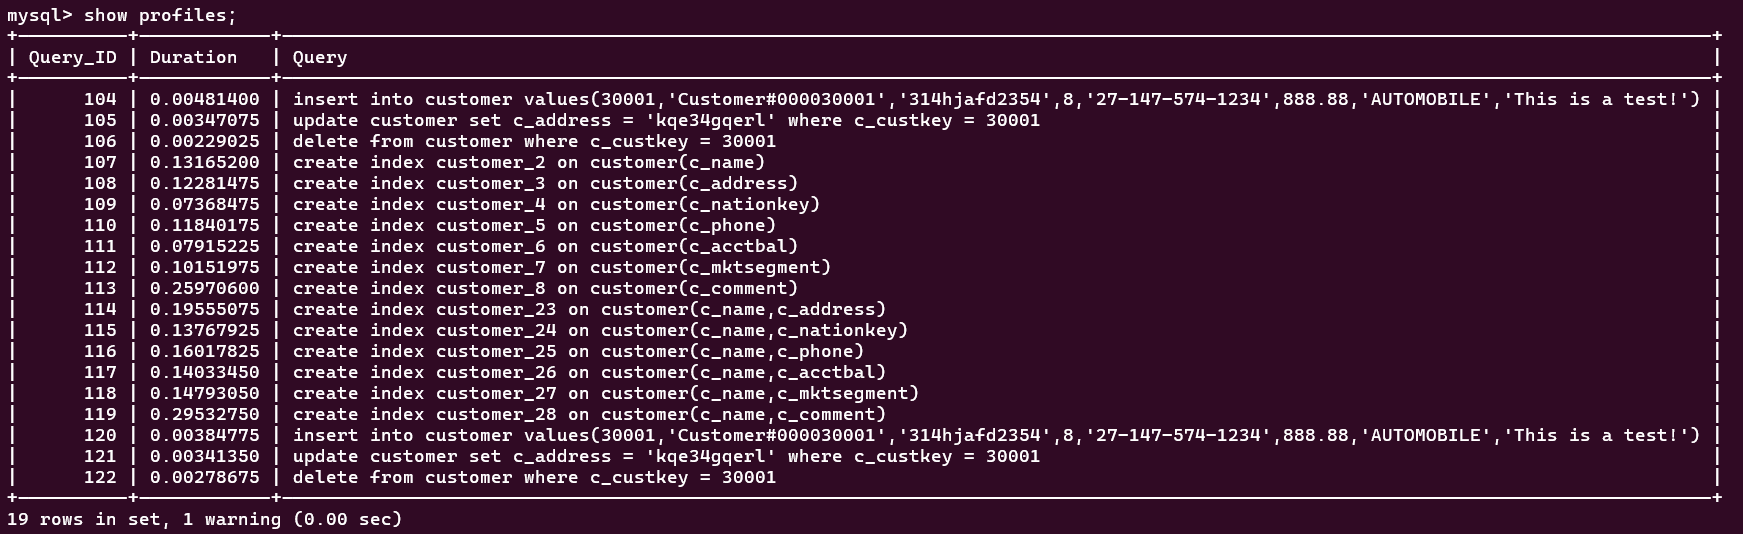
\includegraphics[width=0.9\textwidth]{img/19.png}
\caption{索引对于更新性能的影响}
\end{figure}

可以看到,索引对于更新性能的影响并不明显,因为更新操作主要是对数据表的修改,而索引主要影响查询操作的性能。

\subsection{TPC-H基准测试}

\subsubsection{测试环境}

\begin{itemize}[noitemsep]
  \item \tt{OS: Ubuntu 24.04 LTS on Windows 10 x86\_64}
  \item \tt{Kernel: 5.15.146.1-microsoft-standard-WSL2}
  \item \tt{CPU: 11th Gen Intel i7-11800H (16) @ 2.304GHz}
  \item \tt{Memory: 7832MiB}
  \item \tt{MySQL: 8.2.0}
  \item \tt{PostgreSQL: 16.3 (Debian 16.3-1.pgdg120+1)}
\end{itemize}

\subsubsection{数据集}

\begin{itemize}[noitemsep]
  \item 数据规模:220MB
  \item 索引:默认
\end{itemize}

\subsubsection{测试方法}

先进行2次预热后,进行 5 次测试,取平均值作为最终结果。这样可以尽可能避免冷启动与数据抖动对测试结果的影响。

\subsubsection{测试过程}

依次执行TPC-H的22个查询,记录每个查询的执行时间,并计算总用时。在测试过程中,使用\tt{nmon}工具查看CPU和内存的使用情况并记录。

\subsubsection{测试结果}

查询用时如下表所示:

\begin{longtable}[c]{>{\centering\arraybackslash}p{1.5cm}*{2}{>{\centering\arraybackslash}p{2.5cm}}}
  \caption{查询用时} \\
  \toprule
  \textbf{测试查询} & \textbf{MySQL} & \textbf{PostgreSQL} \\
  & 执行时间(s) & 执行时间(s) \\
  \midrule
  \endfirsthead
  
  \caption[]{(续)} \\
  \toprule
  \textbf{测试查询} & \textbf{MySQL} & \textbf{PostgreSQL} \\
  & 执行时间(s) & 执行时间(s) \\
  \midrule
  \endhead
  
  \midrule \multicolumn{3}{r}{\textit{接下页}} \\
  \bottomrule
  \endfoot
  
  \bottomrule
  \endlastfoot
  
  Q1 & 2.2788 & 0.5588 \\
  Q2 & 0.0966 & 0.0964 \\
  Q3 & 0.4922 & 0.2320 \\
  Q4 & 0.1644 & 0.0500 \\
  Q5 & 0.2599 & 0.0562 \\
  Q6 & 0.3825 & 0.0722 \\
  Q7 & 0.8277 & 0.0666 \\
  Q8 & 0.5842 & 0.0688 \\
  Q9 & 3.5387 & 0.1872 \\
  Q10 & 0.3859 & 0.1118 \\
  Q11 & 0.3572 & 0.0452 \\
  Q12 & 0.5793 & 0.0946 \\
  Q13 & 0.3725 & 0.1356 \\
  Q14 & 0.4602 & 0.0700 \\
  Q15 & 0.4225 & 0.0698 \\
  Q16 & 0.0681 & 0.0834 \\
  Q17 & 313.2492 & 75.3384 \\
  Q18 & 0.5279 & 0.4054 \\
  Q19 & 0.8516 & 0.0972 \\
  Q20 & 475.0988 & 118.2270 \\
  Q21 & 1.0844 & 0.1034 \\
  Q22 & 0.1727 & 0.0488 \\
  \bottomrule
  Total & 802.2555 & 196.2188 \\
  \end{longtable}

CPU和内存使用情况如下表所示:

\begin{table}[H]
  \caption{资源使用情况}
  ~\\
  \centering
  \begin{tabular}{ccc}
    \hline
    \textbf{资源} & \textbf{MySQL} & \textbf{PostgreSQL} \\
    \hline
    CPU & 117\% & 7.17\% \\
    内存 & 96.3\% & 3.8\% \\
    \hline
  \end{tabular}
\end{table}

根据测试结果中的查询用时,以查询为横坐标,执行时间的对数为纵坐标,绘制MySQL和PostgreSQL的查询用时对比图如下:

\begin{figure}[H]
\centering
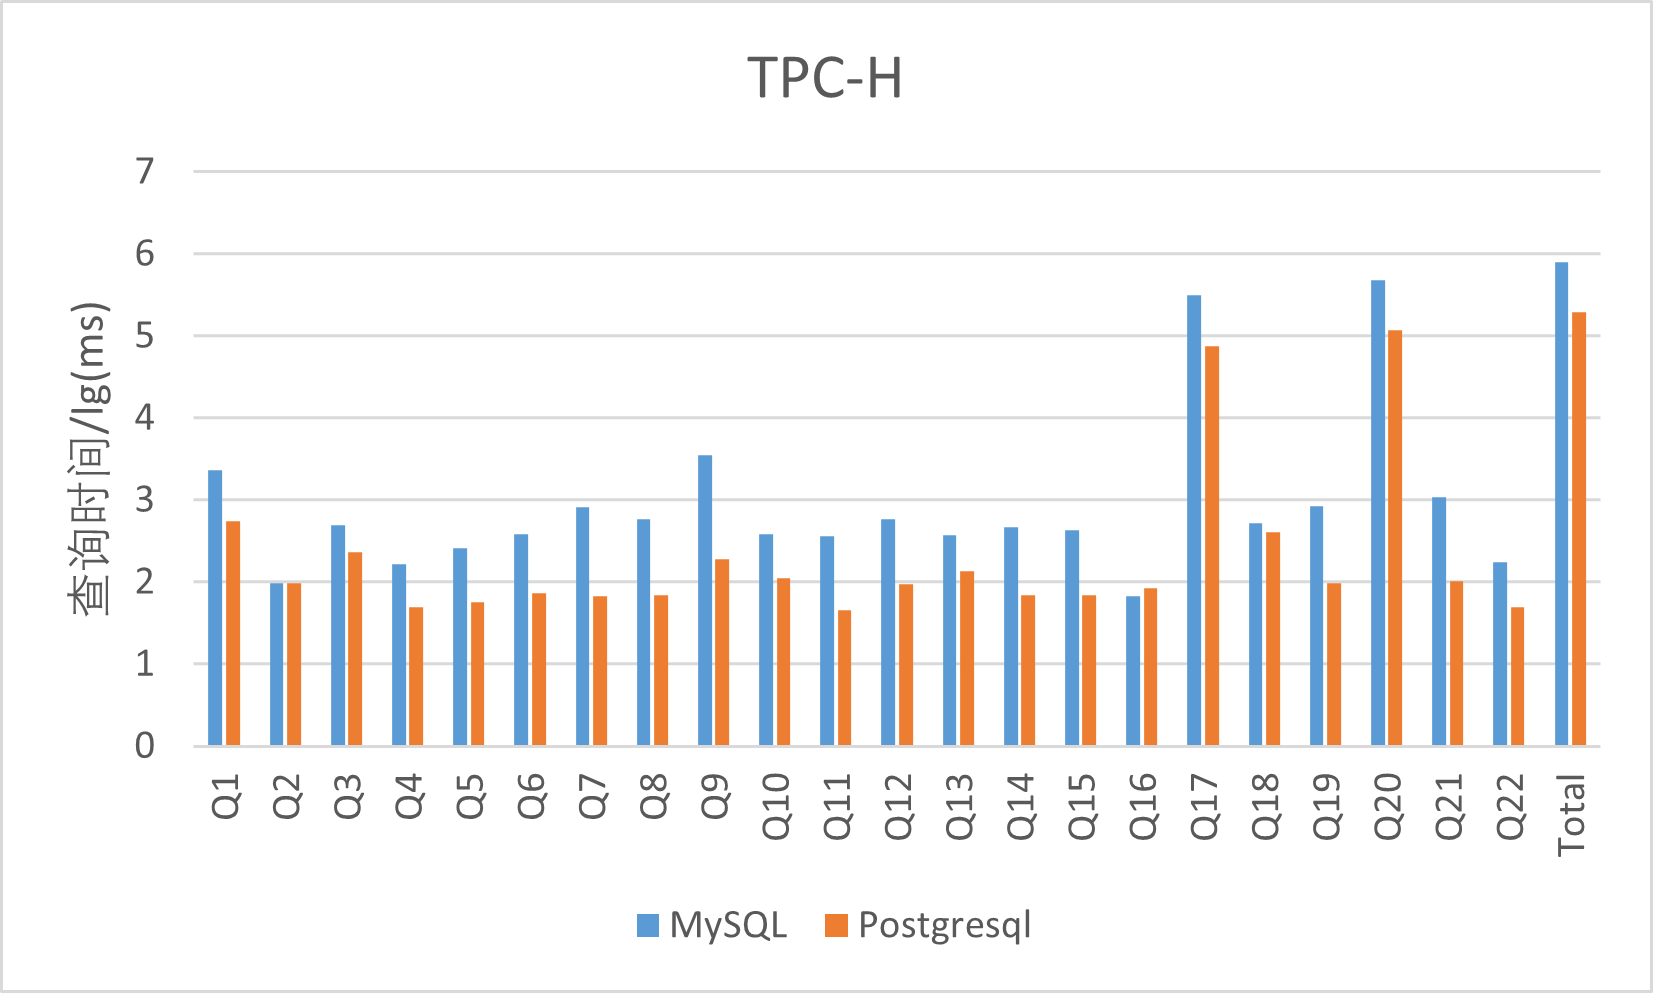
\includegraphics[width=0.9\textwidth]{img/20.png}
\caption{查询用时对比}
\end{figure}

\subsubsection{测试结论}

根据测试结果,可以得出以下结论:

\begin{enumerate}[noitemsep]
  \item 在TPC-H基准测试的查询中,PostgreSQL的执行时间明显优于MySQL,表明PostgreSQL在执行TPC-H基准测试时的性能更好;
  \item PostgreSQL的CPU和内存使用率明显低于MySQL,表明PostgreSQL在执行TPC-H基准测试时的资源消耗更低。
\end{enumerate}

\subsubsection{测试分析}

PostgreSQL在执行TPC-H基准测试时的性能更好,这可能是由于TPC-H基准测试中的查询都比较复杂,PostgreSQL的查询优化器能够更好地优化查询计划,提高查询性能。


\section{存在的问题及解决方案}

\begin{enumerate}
  \item 在使用\tt{drop tablespace} 删除表空间时,提示\tt{ERROR 3120 (HY000): Tablespace `tablespace\_460` is not empty},无法删除表空间;
  
  这是因为表空间中还存在数据表,需要先将数据表迁移到其他表空间,再删除表空间。

  \item 在分析查询资源消耗情况时,以前的查询结果会一直留在 \tt{profiles} 表中;
  
  可以使用以下 SQL 语句清空 \tt{profiles} 表中的数据:

  \begin{lstlisting}[language=sql]
SET @@profiling = 0;
SET @@profiling_history_size = 0;
SET @@profiling_history_size = 100; 
SET @@profiling = 1;
  \end{lstlisting}

  \item 在执行TPC-H基准测试时,使用了其生成的1GB数据集,但在这种数据量下,部分查询需要超过1小时才能完成。因此,为了节省时间,使用了大夏学堂提供的220MB的数据集进行测试。
\end{enumerate}


\section{实验小结}

通过本次实验,我学习了MySQL数据库管理系统中表空间、模式和索引的基本概念和操作,了解了MySQL数据库管理系统中数据存储的基本结构,掌握了索引对查询性能的影响,能够根据应用场景设计合适的索引,同时也学习了使用TPC-H基准测试对数据库管理系统进行评测。通过实验,我对数据库系统的存储、索引和基准测试有了更深入的理解,为今后的数据库系统设计和应用打下了基础。



\end{document}